\documentclass[../../../main.tex]{subfiles}

\begin{document}
    Schließlich untersuchen wir noch das Verhältnis der Pumpleistung $P_p$ und Laserleistung $P_a$. Abbildung zeigt die experimentellen Daten.

    \begin{figure}[H]
        \centering
        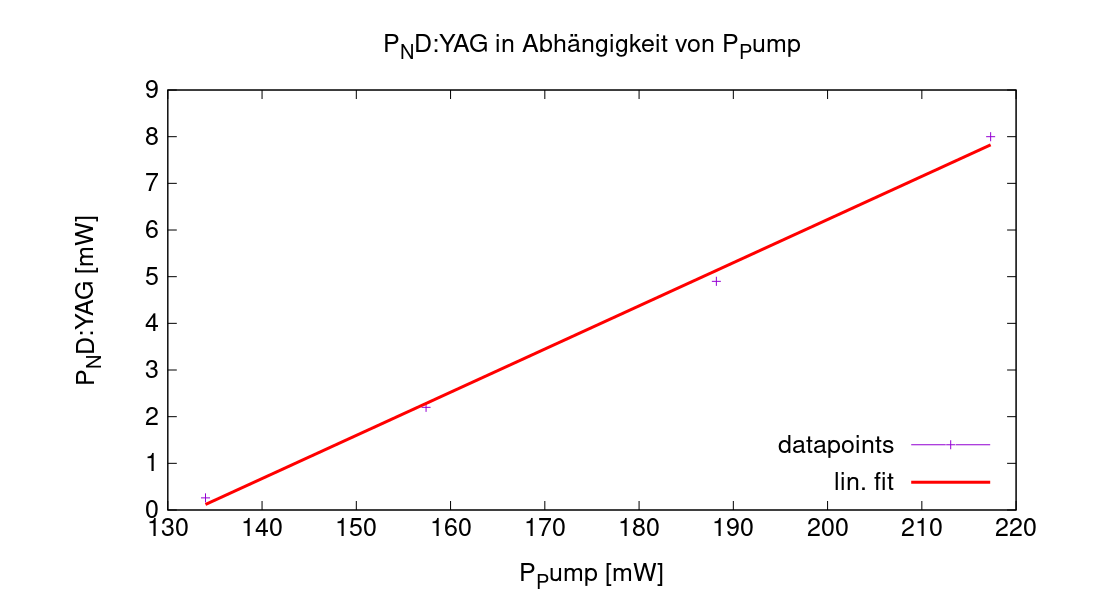
\includegraphics[width=11cm]{../../Bilddateien/5/P(NDYAG)overP(Pump).png}
        \caption{Die Laserleistung $P_a$ als Funktion der Pumpleistung $P_p$}
        \label{fig:PumpLaserLeistung}
    \end{figure}

    Wegen des scheinbar linearen Zusammenhangs wurde ein Fit $f_{a,b} := a\cdot x + b$ durchgeführt, die Parameter sind in Tabelle \ref{tab:PumpLaserLeistungFitParameter} zu sehen.

    \begin{table}[H]
        \centering
        \begin{tabular}{c|cc|cc|cc}
            \hline
             & $a$ in $\si{\m\W}$ & $u(a)$ in $\si{\m\W}$ & $b$ in $\si{\m\W}$ & $u(b)$ in $\si{\m\W}$ \\
            \hline\hline
            $f_{a, b}$ & $0.0925$ & $0.0038$ & $-12.28$ & $0.67$\\
            \hline
        \end{tabular}
        \caption{Die Parameter der exponentiellen Kurvenanpassung.}
        \label{tab:PumpLaserLeistungFitParameter}
    \end{table}

    Es ist also gerade
    \[
        P_{th} = f^{-1}_{a, b}(0) = -\frac{b}{a} = \SI{0.00753(52)}{\m\W}
    \]
    die Laserschwelle, ab welcher Photonenoszillationen im Laser stattfinden. Der theoretische Zusammenhang ist gegeben durch 
    \[
        P_a = \eta\cdot\frac{E_{32}}{E_{41}}\cdot(P_p - P_{th})\cdot \frac{T}{T + L}.
    \]
    Dabei ist $E_{32} = $ das Energieverhältnis der Laserzustände, $E_{41}=$ das Verhältnis der Pumpzustände, $T$ die Transmissivität des Resonatorspiegels und $L$ die sonstige Photonen-Verlustrate. Im verlustfreien Fall gilt $L=0$, also 
    \[
        P_a = \eta\cdot\frac{E_{32}}{E_{41}}\cdot(P_p - P_{th}) \implies eta = \frac{E_{41}}{E_{32}}\cdot \frac{P_a}{P_p - P_{th}}.
    \] 


\end{document}